%!TEX root = ../main.tex

% \section{Computational Model and System Overview}
%\section{Problem Statement and Computational Model}
%\section{Computational Model and System Overview}
\section{Model and System Overview}
\label{sec:problem}
%In this section, we present the formal problem statement and important notations for our approach.
\label{sec:search}
\begin{figure*}[t]
% \vspace{-0.5em}

\centering
% \includegraphics[width=0.5\textwidth]{figures/ov3.pdf}
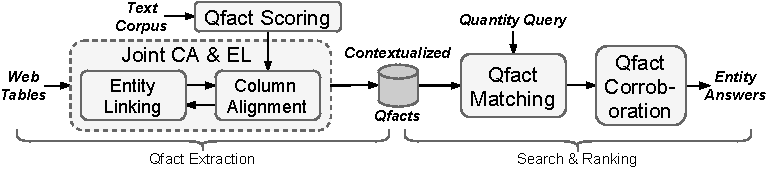
\includegraphics[width=0.7\textwidth]{figures/system_neu4}
% \includegraphics[width=0.75\textwidth]{figures/Qsearch-tables-architecture-11aug2020.pdf}
	\vspace{-0.5em}
\caption{Overview of the 
%Qtables 
QuTE
system.}
%  \vspace{-0.5em}
\label{fig:search_ov}
\end{figure*}

%\subsection{Problem Statement} 
%\noindent{\bf Model:}
\subsection{Model}
%The \textbf{input} of the problem is a \textit{quantity-filter} query (or quantity query) in the form of free text (e.g., 
%% \textit{``Hybrid cars with range on battery more than 50 miles''}, 
%\textit{``Stadiums with capacity more than 70k people''}
% , etc.
%), and a collection of relational web tables, where a relational table is defined as follows:
%GW: already covered in the intro
%
%%%GW introduce and define the key concepts
% web table, qfact, qquery and answer
%

The \textit{input} for fact extraction is a collection of
ad-hoc tables, from a web crawl, spreadsheet corpus
or Wikipedia dump
(e.g., \cite{DBLP:conf/bdc/EberiusBHTAL15}).

%\begin{definition}[Web Table]
\vspace{0.1cm}
\noindent{\bf Definition [Web Table].}
A web table with $r$ rows and
$c$ columns 
% consists of
is a tuple
% of $\mathcal{T} = (\mathcal{H},\mathcal{B}, \mathcal{X})$, where: \\
$T = (H, B, \mathcal{X})$ where:
\squishlist
%\item[-] $r$ and $c$ are two positive integers, denoting the number of rows and columns;
\item[-] ${H} = \{h_i | i \in \{1..c\}\}$ are the headers of the $c$ columns;
%where $h_i$ is the header of the $i$-th column;\\
\item[-] ${B} = \{b_{i,j} | i \in \{1..r\}, j \in \{1..c\}\}$ are cells in the table body;
%where $b_{i,j} $ denotes the cell at body row $i$ and column $j$; \\
\item[-] $\mathcal{X}$ is the context surrounding the table, which typically includes web page title, table caption, DOM-tree headings for the HTML path to the table,
and text in proximity to the table.
\squishend
% We denote $\mathcal{C}_k = \{h_k\} \cup \{b_{i,k} | i \in \{1..r\}\}$ as the $k$-th column of the table, consisting of a header $h_k$ and body cells $\{b_{i,k}\}$. 
% Moreover, we also denote $\mathcal{R}_k = \{b_{k,j} | j \in \{1..c\}\}$ as the $k$-th data row of the table.
We denote ${C}_k = \{h_k\} \cup \{b_{i,k} | i \in \{1..r\}\}$ and ${R}_k = \{b_{k,j} | j \in \{1..c\}\}$ as the $k$-th column and $k$-th row, respectively.
%\end{definition}

\vspace{0.1cm}
This definition is geared for ``horizontal'' tables with column headers and row-wise records. For ``vertical'' tables with row headers and data records per column, we can detect the orientation and apply a
{transpose} operation, using heuristics from \cite{DBLP:journals/pvldb/CafarellaHLMYWW18}.
%\todo{we need to remove "detect the orientation", so reviewers won't ask how to detect}
% \GW{keep this or drop the entire point?}
% \sr{Rewritten with reference I'd lean to keep it}

%Note that the above definition is for tables with horizontal header only (i.e., header is the first row instead of the first column). However, one can easily turn a table with vertical header into this format by using a \textit{``transpose''} operation. In the rest of the paper, we will only stick with this table format.

% \begin{example}
% Sample Table \ref{fig:preprocess_sample_1}-a has number of data rows $r = 4$; number of columns $c = 3$; headers $\mathcal{H} = \{h_1 : \textit{``Team''}, h_2 : \textit{``Stadium''}, h_3 : \textit{``Capacity''}\}$; body cells $b_{1,1} : \textit{``Marseille''}$, $b_{2,3}: \textit{``48,712''}$, etc.; and context caption $\mathcal{X} : \textit{``Stadiums with capacity''}$.
% \qed
% \end{example}

\vspace{0.1cm}
\noindent{\bf Definition [E-column and Q-column].}
For a given table, all columns whose cells 
predominantly contain named entities (which could be
linked to a knowledge base) are referred to as
E-columns. 
All columns whose cells predominantly contain
numeric quantities are denoted as Q-columns.
%
% \vspace{0.1cm}
The implementation of ``predominantly'' is
based on thresholds (say 80\%) for the
fraction of cells that qualify
one way or the other. 
Columns that are neither labeled E nor Q
(e.g., with many cells containing long text)
are disregarded.
%
In Table \ref{table:ExampleTable}, the columns
Team, Stadium and Coach are E-columns, and
Capacity and Value are Q-columns. 

\vspace{0.1cm}

The \textit{output} of extracting facts from a table is represented in the form of triples called 
{quantity facts}, or {\bf Qfacts} for short
(cf. \cite{DBLP:conf/semweb/HoIPBW19} where this terminology is
defined for text-based extraction).

\vspace{0.1cm}
\noindent{\bf Definition [Qfact].}
A quantity fact extracted from table
$T = (H, B, \mathcal{X})$ is a triple of the form
$\mathcal{F} = (e, q, X)$ where:
%%%GW: consider calling them EXQ triples, in contrast to SPO triples
\squishlist
\item[-] $e$ is an entity in a table-body cell $b_{i,j}$ of an
E-column $C_j$, either in the string form of an entity mention or already in the form of a linked entity
uniquely identified in a KB;
\item[-] $q$ is a quantity, properly normalized and with proper unit, in a cell $b_{i,k}$ of a Q-column $C_k$;
\item[-] $X$ is Qfact context, a (small) set of cue words 
(or phrases)
extracted from the table (incl. context $\mathcal{X}$)
that are specifically
informative for the pair $(e, q)$.
\squishend
\vspace{0.1cm}
As an example, a perfect extractor from Table \ref{table:ExampleTable} should produce Qfacts such
as 
(\textit{Estadio Santiago Bernab\'{e}u, 81044,
``stadium, capacity, seats, Madrid''}),
(\textit{Chelsea F.C., 1,958,000,000 GBP,
``team, value, football, London''}),
assuming informative text surrounding the table.

\vspace{0.1cm}
For the downstream use case of query answering, we consider a simple model of telegraphic or question-style
queries containing a single quantity filter,
following \cite{DBLP:conf/semweb/HoIPBW19}:

\vspace{0.1cm}
\noindent{\bf Definition [Qquery].}
A quantity query is a triple $\mathcal{Q} = (qt, qq, qX)$ where:
\squishlist
\item[-] $qt$ is the expected type of answer entities,
such as {\small\tt football team}
or {\small\tt sprinter};
\item[-] $qq$ is a quantity condition of the form ``$\theta ~\textit{value} ~\textit{unit}$'' where $\theta$ can be $\ge$, $\le$, between, or (approximately) equal,
and the unit is optional, as some measures do not have units, such as stadium capacity or country population;
\item[-] $qX$ is a set of additional qualifier terms
that an answer should match, such as ``British'' or ``100 meters'' or ``Olympics'', etc.
\squishend

\vspace{0.1cm}
The \textit{answer} to a Qquery is a Qfact that matches all query conditions, where context terms can be matched approximately (e.g., partially or by embedding-based
similarity):

\vspace{0.1cm}
\noindent{\bf Definition [Qanswer].}
An answer to a Qquery $\mathcal{Q} = (qt, qq, qX)$
is a Qfact $\mathcal{F} = (e, q, X)$ such that
$e$ is an entity of type $qt$,
$q$ satisfies the filter condition $qq$, and
$X$ is a sufficient match to the query context $qX$.
\vspace{0.1cm}

For example, the Qfact 
 (\textit{Chelsea F.C., 1,958,000,000 GBP,
``team, value, football, London''})
would approximately match a query about
``British football teams with value above 1.5 billion pounds'' (as ``British'' and ``London'' are highly
related by word embeddings).

\subsection{System}
%\kp{I changed the flow from here  till 3.4}


%All components of our approach, along with a quantity-query processor and
All components of QuTE, i.e, Qfact extraction method along with a quantity-query processor and
result ranker, are implemented in a 
pipeline depicted in Figure \ref{fig:search_ov}.
%We call our system {\bf QuTE} (for Quantity Table Extraction).
%pronounce: cute
%%%GW: may eventually rename into Qsearch-tables or so
%%%but here, we need to stay double-blind
%%%the name should emphasize the extraction, not the search (yet)

The pipeline starts with quantity recognition and
normalization for Q-columns and
entity linking to a KB for E-columns.
A crucial step then is 
column alignment that links a Q-column
with its proper E-column, to obtain a valid Qfact. %to align a Q-column with its proper E-column, to obtain a valid Qfact. 
%Entity linking and column alignment can be addressed
%by joint inference.
Contextualization and scoring of Qfacts involves
analyzing the 
context
% DOM tree and text 
around a table
and statistics from external corpora. Finally,
query processing involves matching and an additional
scoring step, taking inter-fact consistency into account.

%%%include table pre-processing already here
% For {\bf quantity recognition}, we employ a combination
% of the prior works on QEWT \cite{DBLP:conf/kdd/SarawagiC14} and 
% Illinois Quantifier \cite{DBLP:journals/tacl/RoyVR15}.
% The latter is used to extract numeric values and units from table cells. 
% QEWT is applied to the column headers to discover additional information about units and, possibly, scaling factors. Then, detected quantities are linked to the QuTree catalog~\cite{DBLP:conf/kdd/SarawagiC14} for normalization, including unit conversions.  

%\begin{comment}
%\GW{we have to keep this part, as it is a vital, albeit not original, building block; but we should go back to the previous version's concise text -- ToDo}\\
% \vspace{0.1cm}
% \noindent{\bf Quantity Recognition.}
%
%%%GW{this is old text not in the WSDM submission, which contains many English mistakes - dropped, went back to old WSDM text, don't edit this anymore!!!}
\begin{comment}
For \textbf{quantity recognition}, 
% We preprocess the input table to recognize quantities appearing in table's cells. 
unlike in text, where quantity value and unit go along each other, units of table quantities might appear in the Q-column header. 
Moreover, quantity value could 
% sometimes
be affected by a scaling factor (e.g., thousand, million), also given in the header.

% To recognize quantities in web tables, 
To tackle this,
we employ a combination
of the prior works on QEWT \cite{DBLP:conf/kdd/SarawagiC14} 
% -- providing a table column unit annotator based on a probabilistic context free grammar; 
and Illinois Quantitifer \cite{DBLP:journals/tacl/RoyVR15}.
% -- a tool for extracting quantity from text. 
The latter is used to extract numeric values and units from table body cells $b_{i,j}$. QEWT is applied to the column headers $h_i$ to discover additional information about units and, possibly, scaling factors. 
% If both the header and the body cell provide quantity units, we prioritize using the one given in the header (detected by QEWT), as we observed that units of body cells given by Illinois Quantitier are more noisy.
Then, detected quantities are linked to the QuTree catalog~\cite{DBLP:conf/kdd/SarawagiC14} for normalization, including unit conversions. 
\end{comment}
%
% Detected quantities are linked to the QuTree unit catalog \cite{DBLP:conf/kdd/SarawagiC14}, which provides various units and conversion factors over different measurements, so that they are comparable.

%The latter uses rules to extract numeric values and units
%from table cells. QEWT is applied to the column headers to discover additional information about units and,
%possibly, scaling factors. 
%For normalization, including unit conversions,
%we link detected quantities to the QuTree catalog of
%\cite{DBLP:conf/kdd/SarawagiC14}.
% , that enables comparison between quantities.


%%%GW: here is the polished text from the WSDM submission - fully sufficient!

For {\bf quantity recognition}, we employ a combination
of the prior works on QEWT \cite{DBLP:conf/kdd/SarawagiC14} and 
Illinois Quantifier \cite{DBLP:journals/tacl/RoyVR15}.
The latter is used to extract numeric values and units from table cells. 
QEWT is applied to the column headers to discover additional information about units and, possibly, scaling factors. Then, detected quantities are linked to the QuTree catalog~\cite{DBLP:conf/kdd/SarawagiC14} for normalization, including unit conversions.  

% \vspace{0.1cm}
% \noindent{\bf Entity Recognition.}
For \textbf{entity recognition}, 
% To recognize entities from table body cells $b_{i,j}$,
we employ the
% Stanford NER tool 
% ({\small\url{https://nlp.stanford.edu/software/}})
% and 
AIDA dictionary (\textit{\url{github.com/ambiverse-nlu}}), which provides a large set of entity 
%mentions
names,
such as ``Real'', ``Bayern'', etc.,
and candidate entities.
%along with their candidate entities based on name matches and string similarity, 
%e.g., ``Bayern'':
%{\it Bayern (song)}, 
%{\it Bavaria (Germany)}, 
%{\it FC Bayern Munich}, 
%etc.
%Their disambiguation via entity linking is discussed in Section \ref{sec:extract}.

%\GW{now add a short par on EL here}\\
For {\bf entity linking (EL)} (i.e., disambiguating the recognized mentions onto KB items), there are ample prior works specifically geared for web tables 
\cite{DBLP:journals/pvldb/LimayeSC10, DBLP:conf/semweb/BhagavatulaND15, DBLP:conf/cikm/IbrahimRW16, DBLP:conf/semweb/EfthymiouHRC17, DBLP:conf/edbt/RitzeB17}. We 
%mostly
follow 
\cite{DBLP:conf/semweb/BhagavatulaND15}, with inference
over a probabilistic graphical model. This takes into account a prior for entity popularity, 
context similarity between mentions in table cells and the KB entities, and the coherence among entity candidates for the same row (which should be semantically related entities) and the same column (which should be of the same semantic type). We denote result entities by $\Phi$, with $\Phi(b_{i,j})$ is the entity for input mention $b_{i,j}$ in the table body. 
% For input mentions $b_{ij}$ in the table body, we denote the resulting entities by $\Phi(b_{i,j})$.


%Based on the above steps and using thresholds for
%the per-column fractions, we mark each column either as an {\bf E-column} or a {\bf Q-column} (or as ``none'' in some exceptional cases).
%GW: already said earlier, would be repetition here


